% !TEX encoding = UTF-8 Unicode

\documentclass[twocolumn,10pt,a4j]{ltjsarticle}
\usepackage{kougai}
\usepackage{enumitem}

\title{待ち行列問題シミュレータの開発}
\author{1932008 伊豆原嵩章 指導教員 須田 宇宙 准教授}
\date{}

\begin{document}

\maketitle

\section{はじめに}
病院の受付,店舗や交通渋滞など我々の生活の至る所に待ち行列が存在する.
行列による問題は多岐にわたり生産コストや回転率など,店舗の経営などに大きく関わってくる.
これらは待ち行列問題と呼ばれ,モンテカルロ法を用いてシミュレーションすることが一般的である.

科目「数値計算」の単元に待ち行列問題が存在するが,実際に解こうとしても高い精度の解を算出するために数万回程度の試行が必要となり,手計算での確認は困難である.
そのため,直感的に理解することが困難である.
先行研究では,待ち行列問題を視覚的・直感的に理解するための補助教材としてのシミュレータが存在するが,開発環境が古く現在は使用できないこと,アニメーションが擬似的なものであることなどが問題となっている\cite{past}.

そこで本研究では,アニメーション機能を持ちWebブラウザ上で動作する待ち行列問題シミュレータ教材を開発することを目的とする.


\section{待ち行列問題について}
待ち行列問題とは,$n$箇所の窓口が開いていてサービスに $\delta$時間かかる時の窓口で客がサービスで受けられるまでの平均待ち時間$t$を計算することである.
客はどこかの窓口が空いていればその場所でサービスを受けられるが,全てが使用中だといずれかの窓口が空くまで待たされる.
この待ち時間を集積し全客数で割れば一人当たりの平均待ち時間を計算できる.
$(N+1)$番目の客が入ってくる時刻$t_{N+1}$と個々の客のサービス時間$\delta$は下記の式で表すことができる\cite{text}.
\begin{eqnarray}
t_{N+1} & = & t_N+\tau\\
t_0 & = & 0\\
\tau & = & -\frac{1}{\alpha}\ln\gamma
\end{eqnarray}
(\tau:次の客が入ってくる時間間隔の期待値,\alpha:客の流れの密度,\gamma:区間(0,1)の一様乱数)

%同様に,個々の客のサービス時間$\delta$は以下の式で表せる.
\begin{equation}
\delta=\delta_0+\sigma\nu
\end{equation}
\vspace{-1mm}
($\delta_0$:サービスに必要な平均時間,\sigma:標準偏差,$\nu=\gamma_1+\gamma_2+\cdots+\gamma_{12}-6$)

実際に待ち行列問題を解くためには以下の4つのパラメータを定め,乱数を発生させて計算していく.
\begin{enumerate}
\renewcommand{\labelenumi}{(\roman{enumi})}
\item 客の流れ密度\alpha
\item 窓口の数$n$
\item サービスに必要な平均時間$\delta_0$
\item サービスに必要な時間の標準偏差\sigma
\end{enumerate}


\section{シミュレータ教材について}
図\ref{fig:教科書}は開発したシミュレータ教材のレイアウトである.
過去の卒業研究では問題点であるどのような状況遷移を経てその結果になったか理解することが難しいということから,ユーザーによる入力を行い実行することでアニメーション・グラフの遷移が始まり,状況の遷移を学ぶことできた.
しかし,開発環境が古く現在は使用できないこと,アニメーションが画像を切り替えていくことによる擬似的なアニメーションであり,なめらかなアニメーションではなかった.

そこでアニメーションをより現実的な動きに寄せブラウザ上への移植及び改良することでより利用者の理解度の向上が見込めると考えた.
パラメータの変更はユーザーの任意となっており,パラメータの変化によって待ち行列にどう変化が起こすか学ぶことができる.

①では各パラメータの設定をユーザーによって変更できる.
窓口の平均処理時間(iii)$\delta_0$は1〜10,標準偏差(iv)$\sigma$と流れ密度(i)$\alpha$は0〜1の間で変更できるようにした.
②では平均待ち時間をグラフを表示する.
平均待ち時間の遷移を可視化し,安定状態が理解しやしくなると考えた.
③ではユーザーが設定したパラメータに応じて,アニメーションが実行される.
アニメーションにより現象をより直感的に理解できると考えた.

\begin{figure}[h]
\begin{center}
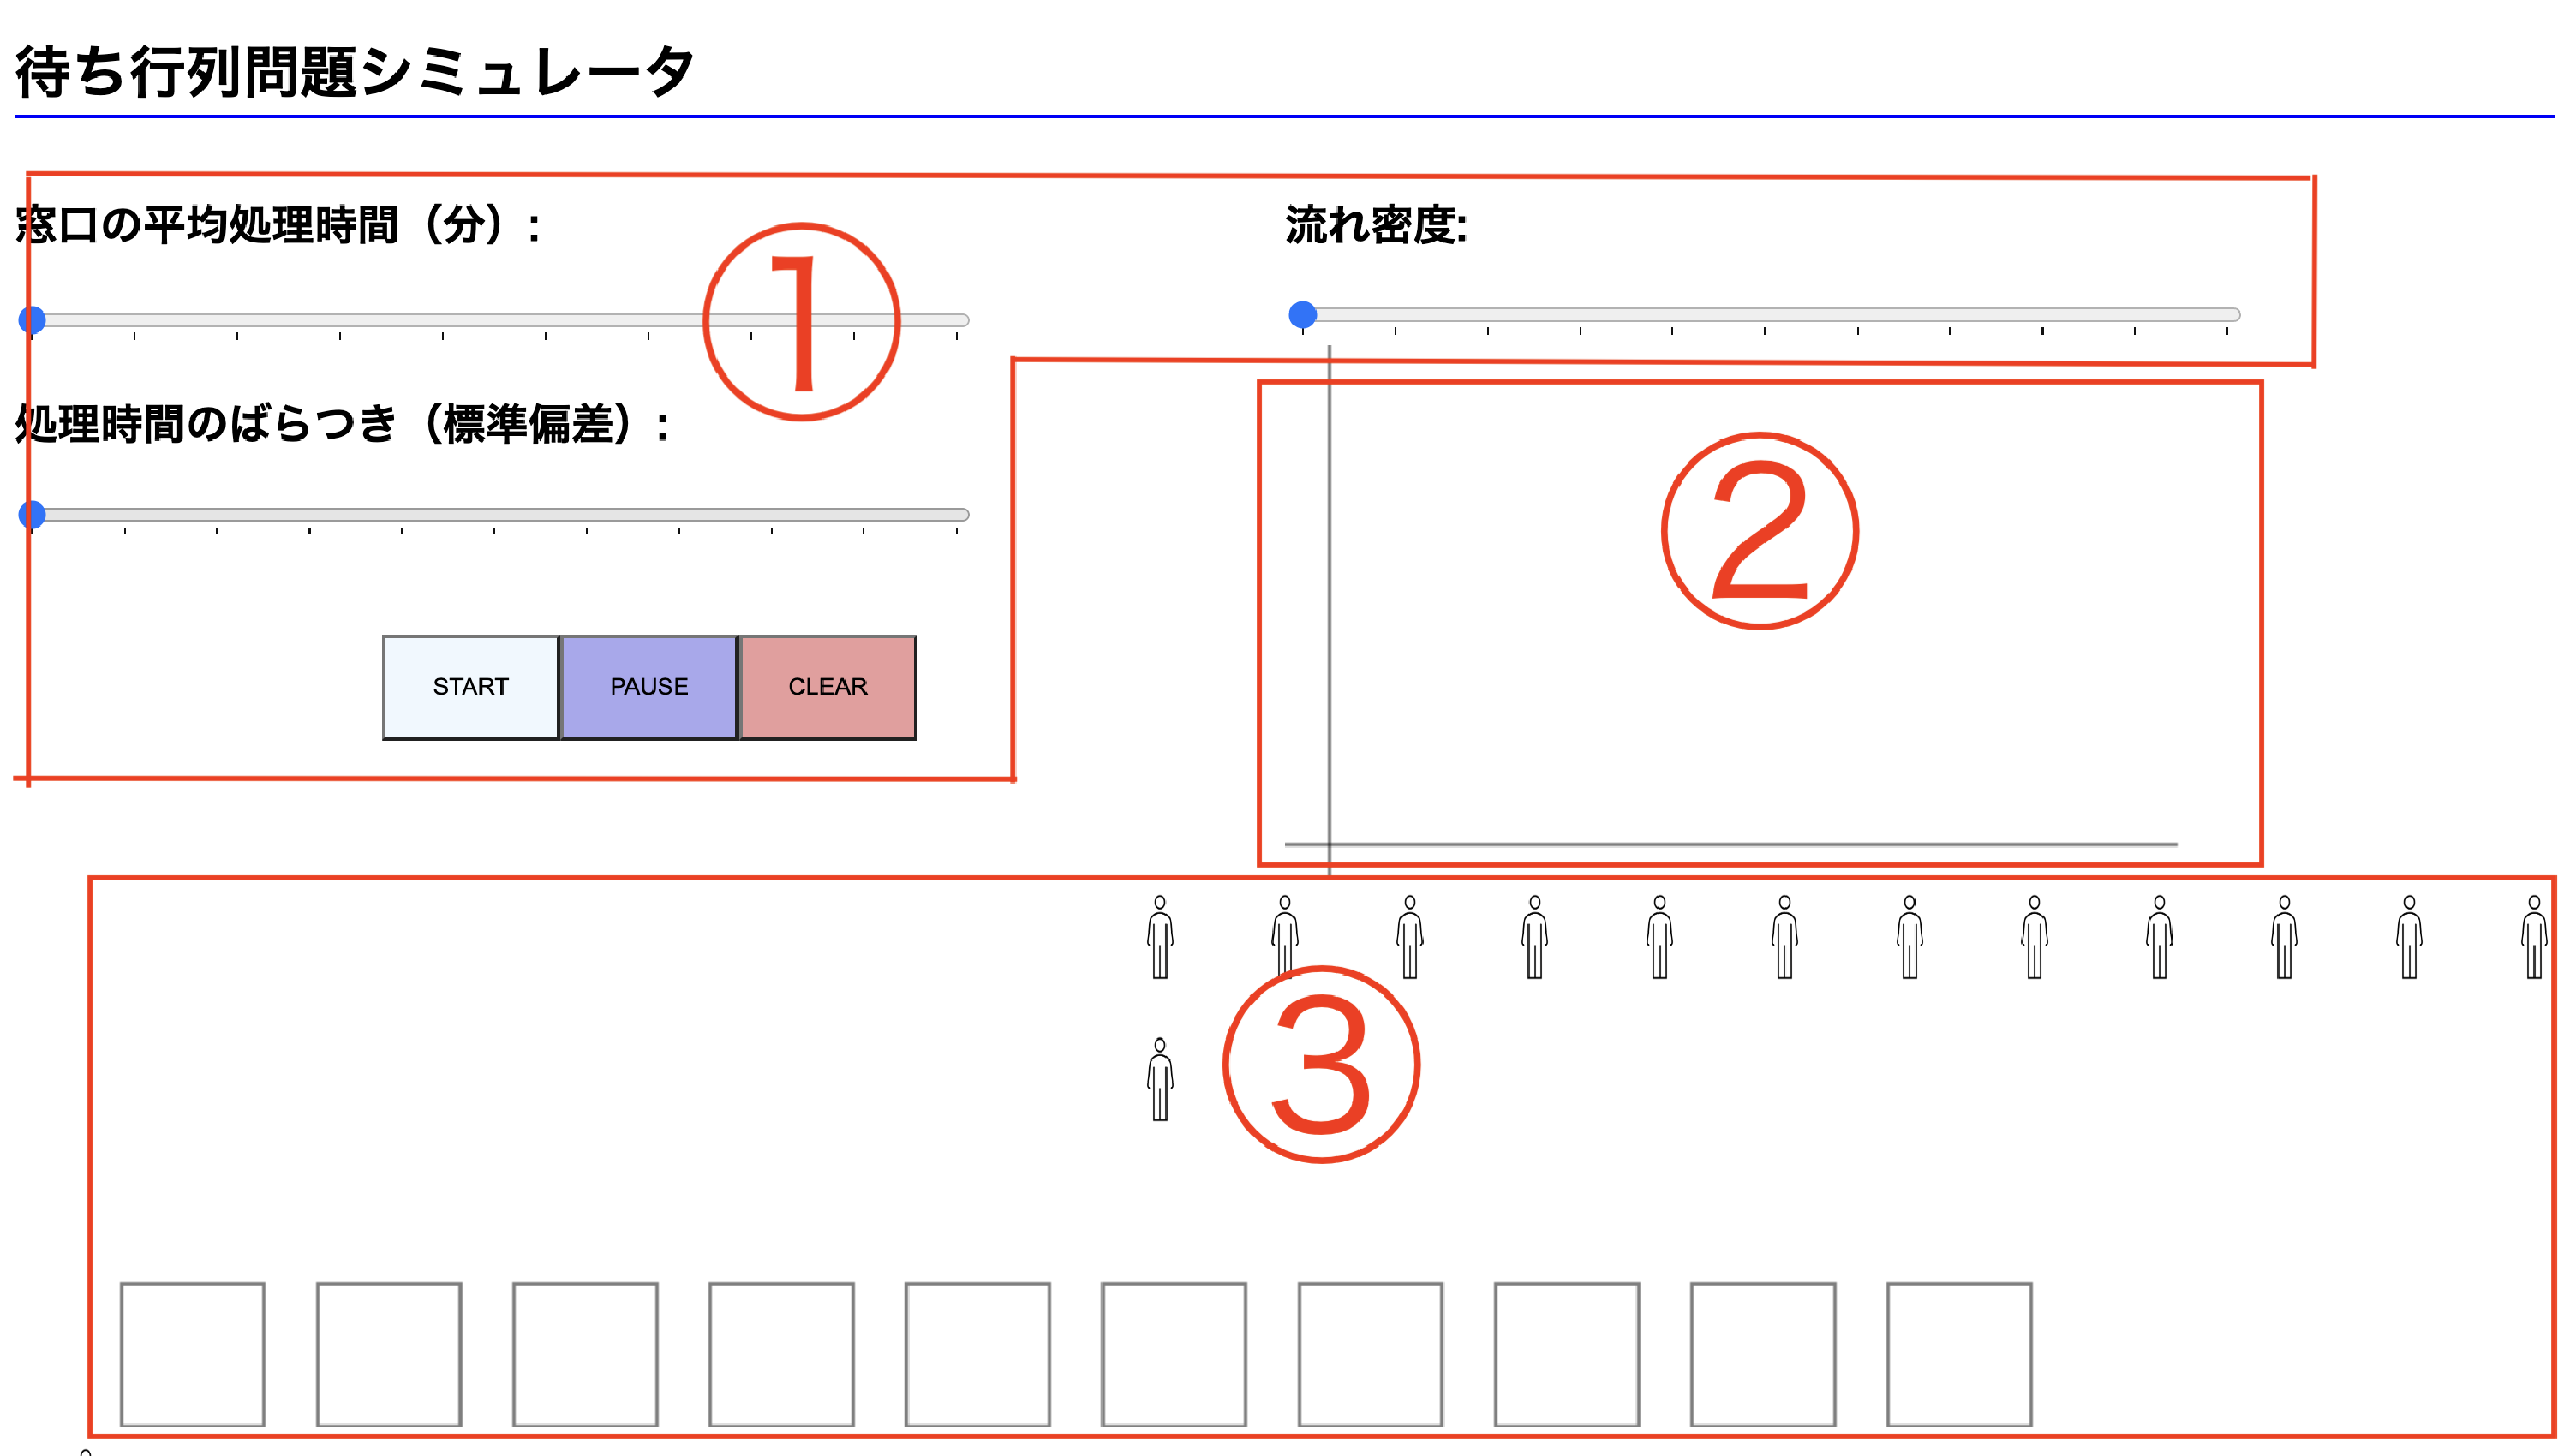
\includegraphics[clip,width=85mm,height=50mm]{figures/layout_ex.pdf}
\end{center}
\caption{シミュレータ教材スクリーンショット}
\label{fig:教科書}
\end{figure}

\section{おわりに}
本研究では,待ち行列についてアニメーションを用いたシミュレータ教材の開発を行った.しかし,技術的な問題で未対応の動作が多く,教材としては不十分なものとなってしまった.

\begin{thebibliography}{99}
\bibitem{past}平成16年度 卒業論文 薄井英彦・梅山卓也 モンテカルロ法による待ち行列問題のマルチメディア教材
 \bibitem{text}第2版 数値計算法 三井田 惇郎・須田 宇宙 共著
\end{thebibliography}
\end{document}
